% Unofficial Umich Poster template.
% A fork of the MSU template https://www.overleaf.com/latex/templates/an-unofficial-poster-template-for-michigan-state-university/wnymbgpxnnwd
% which is a fork of https://www.overleaf.com/latex/templates/an-unofficial-poster-template-for-new-york-university/krgqtqmzdqhg
% which is a fork of https://github.com/anishathalye/gemini
% also refer to https://github.com/k4rtik/uchicago-poster



\documentclass[final]{beamer}

% ====================
% Packages
% ====================

\usepackage[T1]{fontenc}
 \usepackage[utf8]{luainputenc}
\usepackage{lmodern}
\usepackage{threeparttable}
\usepackage{multirow}
\usepackage[size=custom, width=121.92, height=91.44, scale=1.2]{beamerposter}
\usetheme{gemini}
% Custom Harvard Crimson color theme
\definecolor{harvardcrimson}{RGB}{165, 28, 48}
\definecolor{harvardgray}{RGB}{80, 79, 79}
\usepackage{bm}

\setbeamercolor{palette primary}{bg=harvardcrimson,fg=white}
\setbeamercolor{palette secondary}{bg=harvardcrimson,fg=white}
\setbeamercolor{palette tertiary}{bg=harvardcrimson,fg=white}
\setbeamercolor{palette quaternary}{bg=harvardcrimson,fg=white}
\setbeamercolor{structure}{fg=harvardcrimson}
\setbeamercolor{title}{fg=white,bg=harvardcrimson}
\setbeamercolor{headline}{fg=white,bg=harvardcrimson}
\setbeamercolor{footline}{fg=white,bg=harvardcrimson}
\setbeamercolor{block title}{fg=black,bg=white}
\setbeamercolor{block body}{fg=black,bg=white}
\setbeamercolor{block alerted title}{fg=black,bg=harvardcrimson!6}
\setbeamercolor{block alerted body}{fg=black,bg=harvardcrimson!6}
\setbeamercolor{alerted text}{fg=harvardcrimson}
\usepackage{graphicx}
\usepackage{booktabs}
\usepackage{tikz}
\usepackage{pgfplots}
\pgfplotsset{compat=1.14}
\usepackage{anyfontsize}
\usepackage{qrcode}   % <-- moved here, after pgfplots

% ====================
% Lengths
% ====================

% If you have N columns, choose \sepwidth and \colwidth such that
% (N+1)*\sepwidth + N*\colwidth = \paperwidth
\newlength{\sepwidth}
\newlength{\colwidth}
\setlength{\sepwidth}{0.025\paperwidth}
\setlength{\colwidth}{0.3\paperwidth}

\newcommand{\separatorcolumn}{\begin{column}{\sepwidth}\end{column}}

\newcommand{\blockrule}{\vspace{-1.5em}\textcolor{harvardcrimson}{\rule{\linewidth}{1.2pt}}\vspace{-0.2em}}

% ====================
% Title
% ====================

\title{Variational Boosting for Physics-Informed Neural
Networks}

\author{Kaylee Vo \and Pavlos Protopapas}

\institute[shortinst]{Harvard John A. Paulson School of Engineering and Applied Sciences}

% ====================
% Footer (optional)
% ====================

\footercontent{
  \href{https://github.com}{Github: https://github.com/kayleeisokay} \hfill
STAI-X 2026 Poster Session \hfill
  \href{mailto:kav418@g.harvard.edu}{kav418@g.harvard.edu}}
% (can be left out to remove footer)

% ====================
% Logo (optional)
% ====================

% use this to include logos on the left and/or right side of the header:
% Left: institution
 % \logoright{
\includegraphics[height=8cm]{logos/seas_logo.png}}
% Right: funding agencies and other affilations 
%\logoright{\includegraphics[height=7cm]{logos/NSF.eps}}
% ====================
% Body
% ====================

% use this to include logos on the left and/or right side of the header:
% Left: institution
\logoleft{\qrcode[height=8cm]{https://kayleeisokay.github.io/}}
% Right: funding agencies and other affilations 
\logoright{
\includegraphics[height=8cm]{logos/seas_logo_bw.png}}

\begin{document}



\begin{frame}[t]
\begin{columns}[t]
\separatorcolumn

\begin{column}{\colwidth}

  \begin{block}{Introduction}
    \blockrule
    
    Physics-Informed Neural Networks (PINNs) solve differential equations by minimizing a residual functional $\mathcal{L}(u) = \|F(u)\|^2$ over a neural parameterization $u_\theta$. Monolithic PINNs, however, suffer from \textbf{ill-conditioning}, \textbf{spectral bias}, and \textbf{optimization instability} when a single network must learn all scales of a solution at once.

    We introduce a variational boosting framework \cite{fang-2023} in which solutions are constructed additively in function space. Each stage trains a weak learner whose converged correction satisfies a local orthogonality condition, equivalent to a \textbf{projected functional gradient descent step} onto the tangent space of the network's function manifold. Because each correction network is deliberately small, the restricted minimization admits  \textbf{full Newton} or \textbf{conjugate gradient} (CG) updates. 

  \end{block}
    \vspace{-0.5em}
  \begin{block}{Motivation}
    \blockrule
    
    The functional gradient of the residual is
    $
      \nabla_u \mathcal{L}(u) = 2\,F'(u)^{*}F(u),
    $
    where $F'(u)$ is the Fr\'echet derivative of the operator $F$ and $F'(u)^*$ its adjoint. For nonlinear operators, this linearization evolves as $u$ changes during training, so the curvature of the loss landscape shifts throughout optimization.

    \textbf{Boosting} addresses this by separating the learning task across stages: each small network is individually well-conditioned, avoiding the need to learn all scales simultaneously.

  \end{block}
    \vspace{-1em}
  \begin{alertblock}{Contributions}
    \blockrule
    
    \begin{enumerate}
      \item A theoretical, geometric interpretation of multi-stage PINNs as
        \textbf{projected functional descent step}.
      \item \textbf{Second-order optimization} using full Newton and CG.
      \item \textbf{Transfer learning} across correction stages.
    \end{enumerate}

  \end{alertblock}
    \vspace{-1em}
  \begin{block}{Boosted PINN Framework}
    \blockrule
    
    The solution is built as an \textbf{additive ensemble}. Stage 0 is a standard PINN trained on the full problem, giving $u^{(0)} = h_0$. Each subsequent stage $k \geq 1$ trains a small weak learner $h_k$ to reduce the residual left by the current ensemble, and updates:
\begin{equation}
  u^{(k)} = u^{(k-1)} + \alpha_k h_k,
\end{equation}
where $\alpha_k > 0$ is a shrinkage parameter. After $K$ stages, $u^{(K)} = h_0 + \sum_{k=1}^{K}\alpha_k h_k$. The steepest descent direction at $u^{(k-1)}$ is
\begin{equation}
  -\nabla_{\mathcal{H}}\mathcal{L}(u^{(k-1)}) = -2\,F'(u^{(k-1)})^{*}\,r^{(k-1)},
\end{equation}
where $r^{(k-1)}$ is the current residual and $F'(u^{(k-1)})^{*}$ is the adjoint of the linearized operator. Training $h_k$ to minimize the updated residual is \emph{approximately} equivalent to finding the element of $\mathcal{U}_k$ that best matches this steepest-descent direction. 
\vspace{-0.5em}
\begin{itemize}
    \item Linearizing $F$ and minimizing the resulting residual gives a Gauss–Newton step, which generally differs from steepest descent. 
    \item Training directly on the full nonlinear residual is neither, since $F$ is re-evaluated at the moving iterate throughout training.
\end{itemize}

    \begin{figure}
      \centering
      
\includegraphics[width=1.0\textwidth]{plots/ode/duffing/weak_learners.png}
      \caption{Weak learners $h_k$ shrink toward zero as the residual is
      reduced (Duffing equation).}
    \end{figure}

  \end{block}

\end{column}

\separatorcolumn

\begin{column}{\colwidth}

  

  \begin{block}{Second-Order Optimization}
    \blockrule
    
    \begin{itemize}
      \item \textbf{Conjugate Gradient}: solves $(H+\gamma I)d = -g$ using only Hessian--vector products, avoiding explicit formation of $H$.
      \item \textbf{Newton's Method}: computes $H$ explicitly, uses Tikhonov regularization when $H$ is not positive-definite, and applies trust-region step-size control..
      \item Implementation: \textbf{Adam $\to$ second-order optimizer} ($\sim$90\% Adam, then CG/Newton) lets Adam reach a well-conditioned region before exploiting local curvature.
    \end{itemize}

    \begin{table}[ht]
    \centering
    \begin{tabular}{lccc}
        \toprule
        & \textbf{Monolithic PINN} & \multicolumn{2}{c}{\textbf{Boosted PINN}} \\
        \cmidrule(lr){2-2} \cmidrule(lr){3-4}
        Metric & L-BFGS & Adam + CG & Adam + Newton \\
        \midrule
        Residual Norm         & $3.88 \times 10^{-3}$ & $5.43 \times 10^{-3}$ & $\bm{3.24 \times 10^{-3}}$ \\
        MSE                   & $3.77 \times 10^{-4}$ & $7.08 \times 10^{-4}$ & $\bm{1.44 \times 10^{-4}}$ \\
        Relative $L^2$ Error  & $6.19 \times 10^{-4}$ & $9.64 \times 10^{-4}$ & $\bm{2.17 \times 10^{-4}}$ \\
        Training Time (s)     & $\bm{0.31}$           & $7.03$                & $187.72$              \\
        Number of Iterations  & $\bm{132}$            & $738$                 & $407$                 \\
        Learning Rate         & $1.00$                & $0.01$                & $0.01$                \\
        Collocation Points    & $1{,}000$             & $1{,}000$             & $1{,}000$             \\
        Network Size          & $2{,}209$             & $2{,}209$             & $2{,}209$             \\
        \bottomrule
    \end{tabular}
    \caption{Monolithic vs.\ Boosted PINN performance on the Duffing equation.}
    \label{tab:duffing_comparison}
    \end{table}

  \end{block}
\vspace{-1em}
  \begin{block}{Warm-Start Via Transfer Learning}
    \blockrule
    
    Each $h_k$ is initialized by transferring weights from $h_{k-1}$,
    with the final two layers re-initialized (Xavier) and rescaled by a
    stage-specific factor $\xi_k$. Removing transfer learning
    significantly degrades performance --- e.g.\ MSE on Lotka--Volterra
    worsens from $1.76\times10^{-3}$ to $7.91\times10^{-1}$
    ($p = 0.0042$).

  \end{block}
    \vspace{-0.7em}
  \begin{alertblock}{Results Summary}
  \blockrule

    Across ODE, coupled-ODE, and PDE benchmarks, the boosted PINN
    \textbf{matches or exceeds} standard (monolithic) PINN accuracy and converges where standard PINNs \textbf{fail outright}, an advantage especially pronounced in stiff regimes.

    \begin{table}
      \centering
      \small
      \begin{tabular}{lccc}
        \toprule
        \textbf{Problem} & \textbf{Std.\ PINN MSE} & \textbf{Boosted MSE} & \textbf{Converges?} \\
        \midrule
        Duffing            & $3.77\times10^{-4}$ & $1.44\times10^{-4}$ & Both \\
        NRD ($\kappa{=}100$, stiff)  & $9.27\times10^{-1}$ & $8.01\times10^{-3}$ & Boosted only \\
        Van der Pol ($\mu{=}3$) & --- & $5.71\times10^{-3}$ & Boosted only \\
        Lotka--Volterra    & $1.74\times10^{-2}$ & $2.92\times10^{-3}$ & Boosted only \\
        Burgers' (\nu = 0.002)  &  $9.27 \times 10^{-1}$  & $5.36 \times 10^{-2}$ & Neither \\
        Allen--Cahn (D=0.0001) & $1.41\times10^{-2}$ & $7.10\times10^{-3}$ & Boosted only \\
        \bottomrule
      \end{tabular}
      \caption{Selected MSE comparison (best optimizer per model). ``---'' = did not converge.}
    \end{table}

    \begin{table}[H]
    \centering
    \begin{threeparttable}
    \begin{tabular}{llcc}
        \toprule
        \textbf{Problem} & \textbf{Method} & \textbf{Iterations} & \textbf{Wall-Clock} \\
        \midrule
        \multirow{3}{*}{Duffing}
            & Adam          & $2.18\times$ & $0.40\times$ \\
            & Adam + CG     & $2.07\times$ & $0.46\times$ \\
            & Adam + Newton & $3.76\times$ & $0.02\times$ \\
        \midrule
        Allen--Cahn (nonstiff) & Adam & $1.00\times$ & $1.26\times$ \\
        \bottomrule
    \end{tabular}
    \caption{Convergence metrics for boosted PINN vs.\ standard, restricted to problems where both converged (Higher favors boosted PINN).}
    \label{tab:speedup_summary}
    \end{threeparttable}
\end{table}
\vspace{-0.5em}
Standard PINN failed to converge on: NRD equation (both stiff and nonstiff), Van der Pol equation, Lotka--Volterra coupled ODE system, Allen--Cahn equation (stiff), Burgers' equation (stiff and nonstiff). Our \textbf{method converges quicker} than other ensemble methods \cite{inproceedings}, uses \textbf{smaller models}, and yields performance on the same order of magnitude.  

  \end{alertblock}

\end{column}

\separatorcolumn

\begin{column}{\colwidth}

  

  \begin{alertblock}{Stiff PDE Example (Allen-Cahn)}
    \blockrule
    \begin{figure}
      \centering
      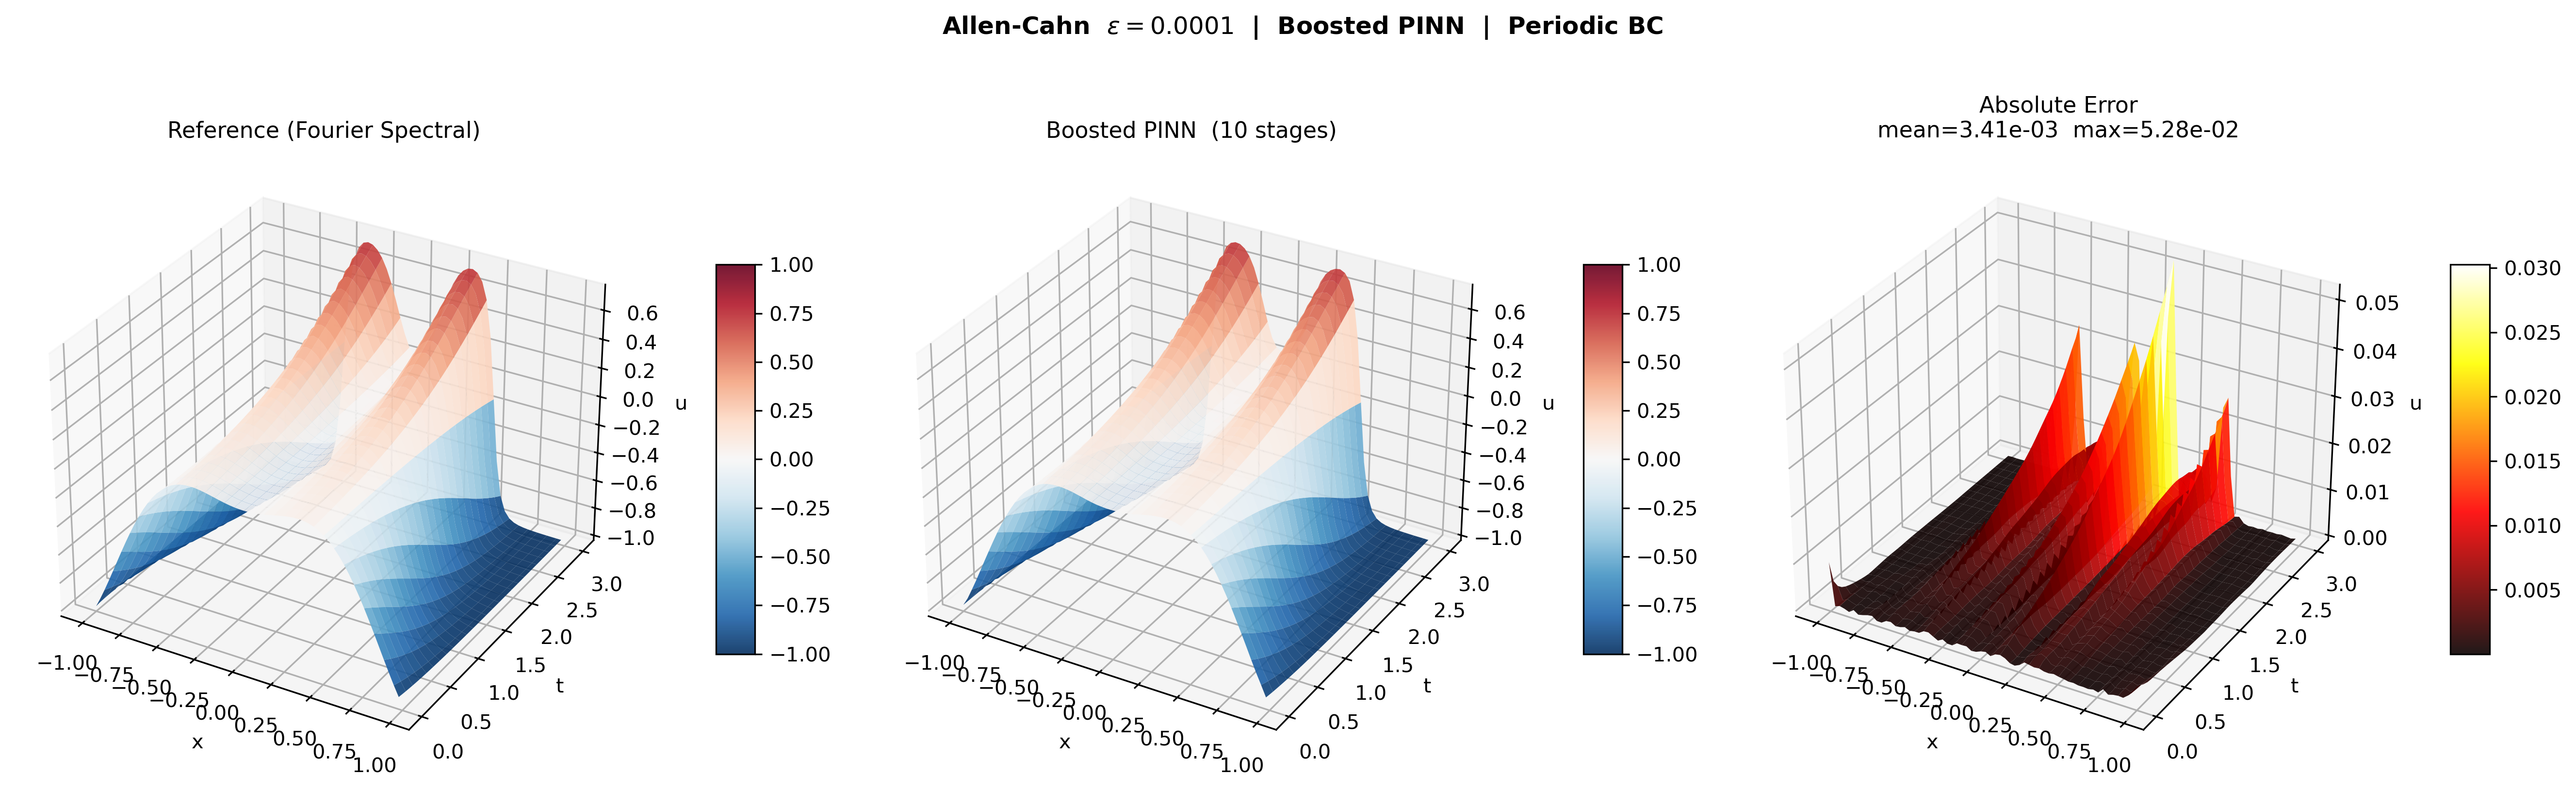
\includegraphics[width=0.9\textwidth]{plots/pde/allen-cahn/D0.0001/solution_3d_comparison.png}
      \caption{Boosted PINN solution cross-sections to the Allen--Cahn PDE (D=0.0001).}
    \end{figure}

    \begin{figure}
      \centering
      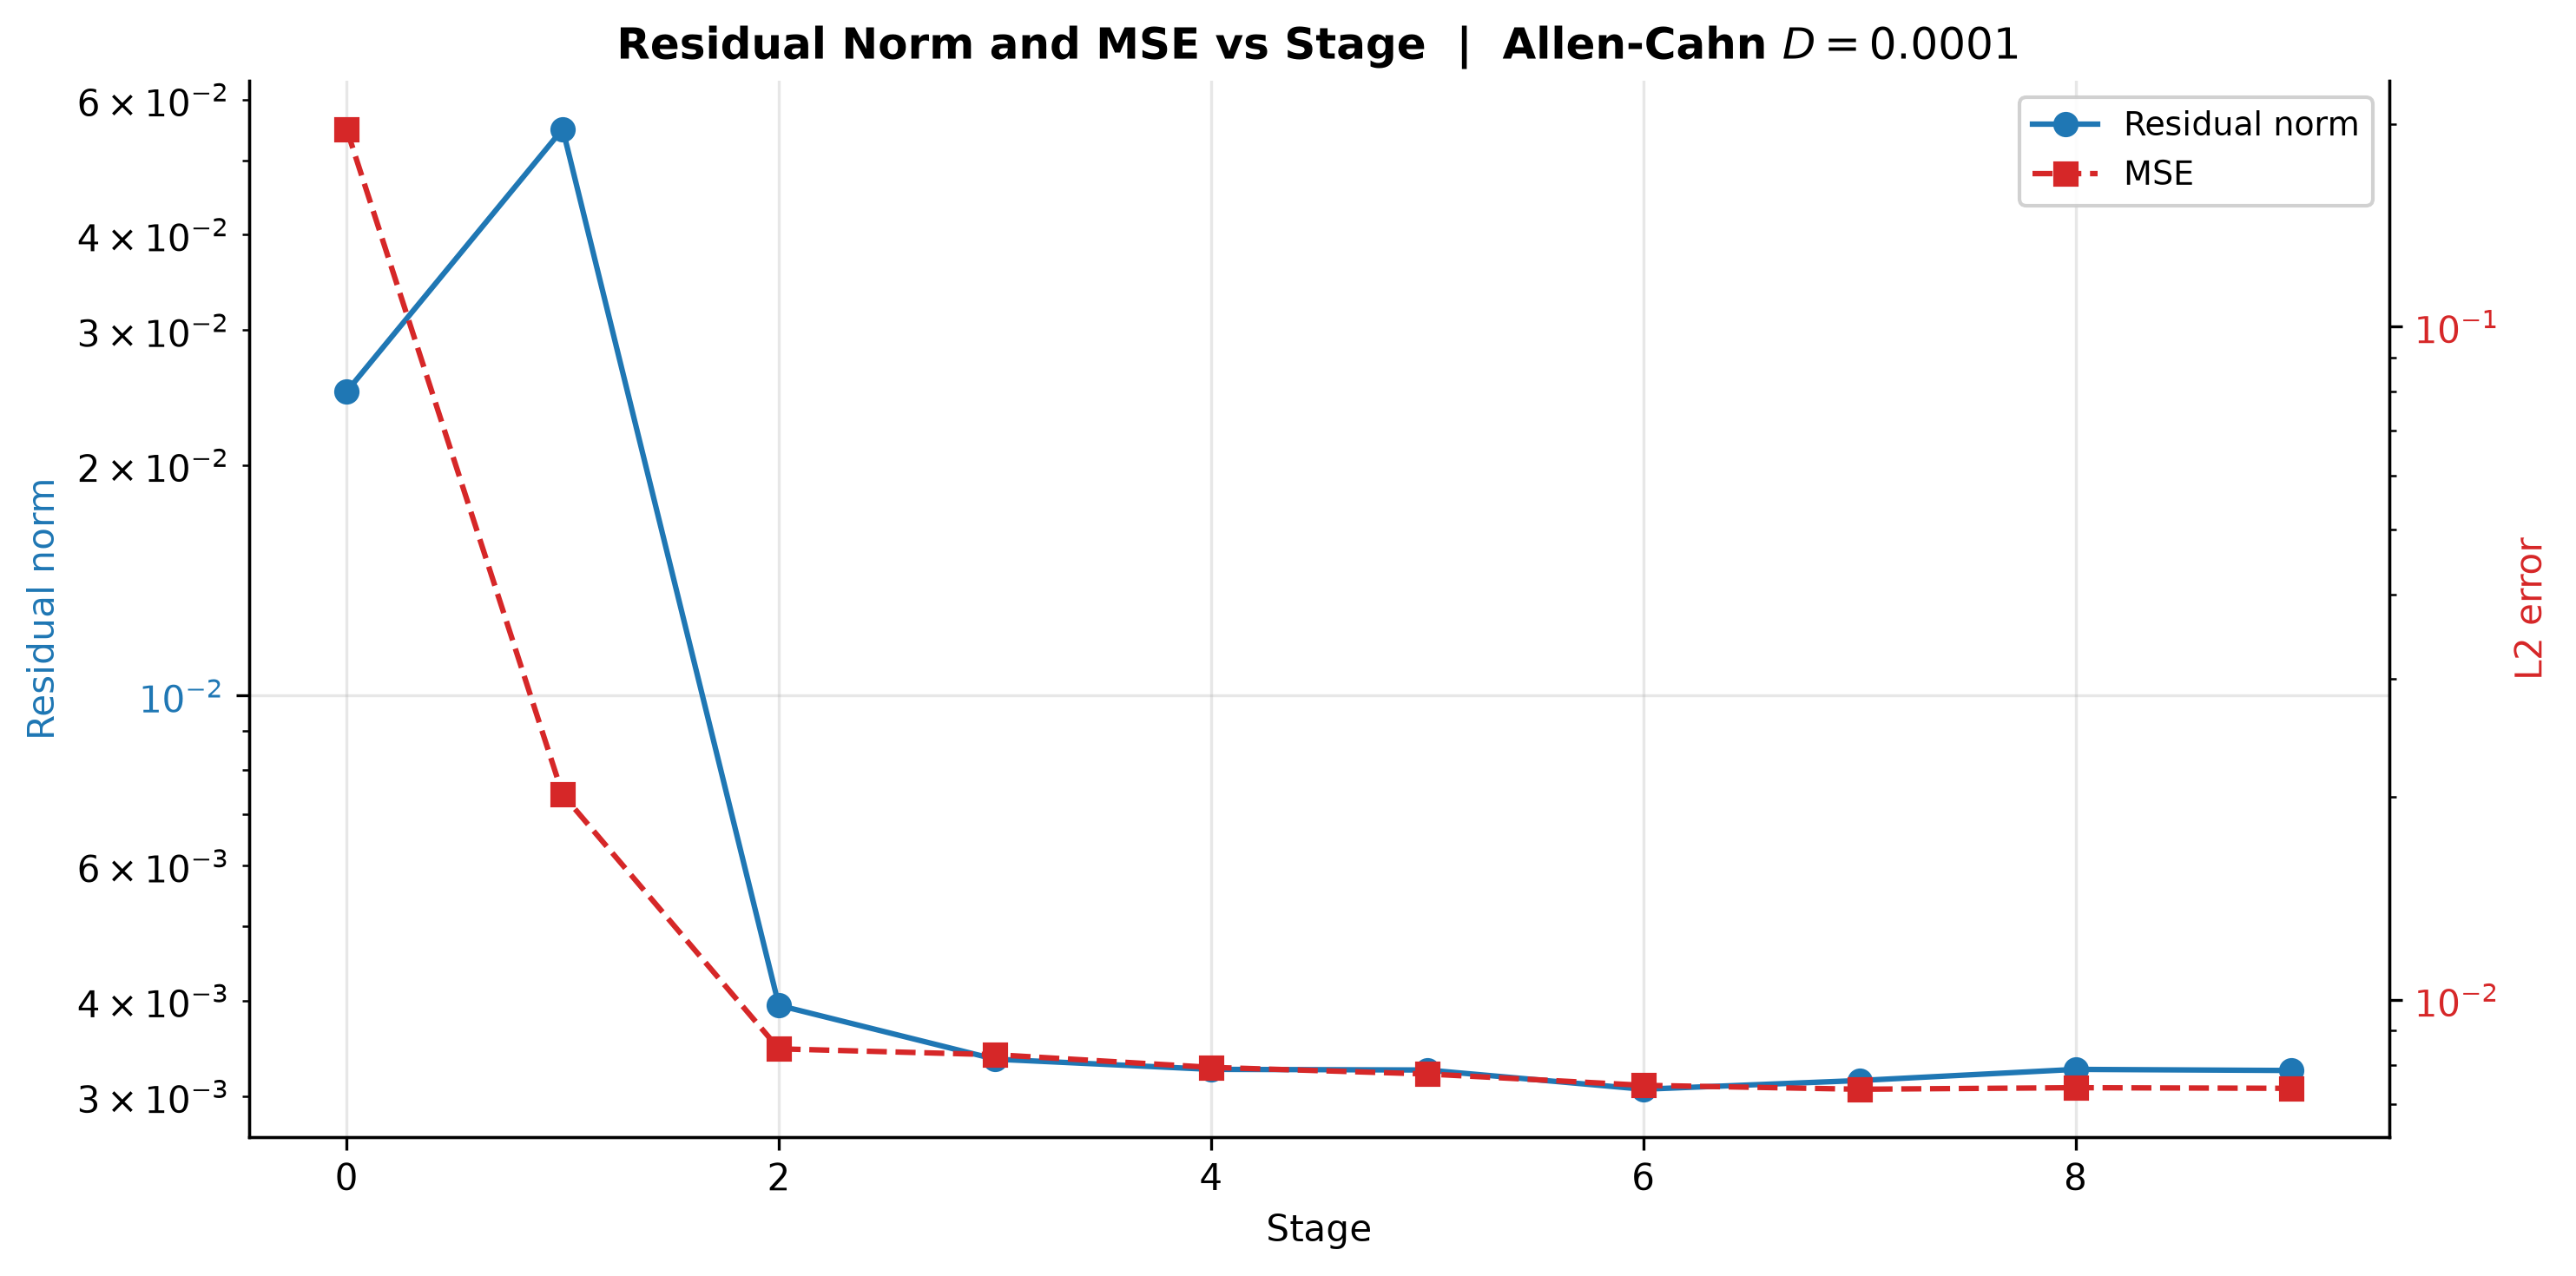
\includegraphics[width=0.6\textwidth]{plots/pde/allen-cahn/D0.0001/residual_l2_vs_stage.png}
      \caption{Residual and MSE across stages for Allen--Cahn PDE (D=0.0001).}
    \end{figure}

  \end{alertblock}
    \vspace{-1.0em}
  \begin{block}{Sensitivity \& Limitations}
    \blockrule
  \begin{figure}
      \centering
      
\includegraphics[width=0.8\textwidth]{plots/sensitivity_analysis/coupled_ode/heatmap_l2_error.png}
      \caption{Sensitivity heatmap for Lotka--Volterra}
    \end{figure}
    \vspace{-1em}
    \begin{itemize}
      \item \textbf{More stages / larger weak learners} $\to$ lower MSE for nonstiff problems (e.g.\ Lotka--Volterra), but for stiff PDEs (Allen--Cahn) an \textbf{intermediate} hidden size (64--128) performs best --- oversized weak learners re-introduce spectral bias.
      \item Boosting has a stiffness ceiling. Converges for Van der Pol
        when $\mu = 3$ but not for $\mu = 4$. Fails for Burgers' ($\nu = 0.002$). Boosted PINNs also suffer from long temporal issues as traditional PINNs.
      \item Second-order optimizers are currently validated only on
        \textbf{nonstiff ODEs}; extending to stiff PDEs is future work.
    \end{itemize}

  \end{block}
    \vspace{-1em}
  \begin{block}{References}
    \blockrule
    \nocite{*}
    \footnotesize{\bibliographystyle{plain}\bibliography{poster}}

  \end{block}

\end{column}

\separatorcolumn
\end{columns}
\end{frame}

\end{document}